\documentclass[twosided,a4,10pt]{article}
\usepackage[utf8]{inputenc}
\usepackage{amsmath}
\usepackage{amsfonts}
\usepackage{amssymb}
\usepackage{amstext}
\usepackage{mathrsfs}
\usepackage{textcomp}
\usepackage{german}
\usepackage{graphicx}
\usepackage[usenames,dvipsnames]{xcolor}
\usepackage{pifont}
\usepackage{nicefrac}
\usepackage{sectsty}
\usepackage{dblfnote}
\usepackage{verbatim}
% ------
% Fonts and typesetting settings
\usepackage[sc]{mathpazo}
\usepackage[T1]{fontenc}
\linespread{1.1} % Palatino needs more space between lines
\usepackage{microtype}
\subsectionfont{\fontsize{10}{15}\selectfont}

% ------
% Page layout
\usepackage[hmarginratio=1:1,top=32mm,columnsep=20pt]{geometry}
\usepackage[font=it]{caption}
\usepackage{paralist}
\usepackage{multicol}

%--------
%Footnote
\usepackage{footnote}
\usepackage{perpage} %the perpage package
\MakePerPage{footnote} %the perpage package command
\addtolength{\skip\footins}{2pc plus 5pt}
%------
%caption hack
\usepackage{caption}

%\DeclareCaptionType{faltung}[][List of equations]
%\captionsetup[faltung]{labelformat=empty}

% ------
% Abstract
\usepackage{abstract}
\renewcommand{\abstractnamefont}{\normalfont\bfseries}
\renewcommand{\abstracttextfont}{\normalfont\small\itshape}


% ------
% Titling (section/subsection)
\usepackage{titlesec}
%\renewcommand\thesection{\Roman{section}}
\titleformat{\section}[block]{\large\scshape\centering}{\thesection.}{1em}{}

% ------
% Clickable URLs (optional)
\usepackage[hyphens]{url}
\usepackage{hyperref}

% ------
% Header/footer
\usepackage{fancyhdr}
\pagestyle{fancy}
%	\fancyhead{}
%	\fancyfoot[C]{WIS WS 2017/18 $\cdot$
% Software Engineering $\cdot$ Prof. Dr. Dünnweber}
\fancyhead[R]{OTH Regensburg $\cdot$ Fakultät IM}
%	\fancyfoot[RO,LE]{\thepage}
\fancyfoot[L]{WIS $\cdot$ WS 2017/18}
\fancyfoot[R]{Prof. Dr. Dünnweber}
\fancyfoot[C]{\thepage}


% ------
% Maketitle metadata
\title{\vspace{-5mm}%
	\fontsize{20pt}{10pt}\selectfont
	\textbf{Inhaltsbasierte Musikempfehlung mit Convolutional Neuronalen Netzwerken}
}	
\vspace{-5mm}\date{}
\author{
	\large\begin{minipage}[t]{0.5\linewidth}
		\begin{center}
			\textsc{Weidhas Philipp}\\[2mm]
			\normalsize	Matr.nr: 123456\\
			\normalsize
			\href{mailto:philipp.weidhas@st.oth-regensburg.de}
			{philipp.weidhas@st.oth-regensburg.de}
		\end{center}
	\end{minipage}
	\begin{minipage}[t]{0.5\linewidth}
		\begin{center}
			\textsc{Wildgruber Markus}\\[2mm]
			\normalsize	Matr.nr: 123456\\
			\normalsize
			\href{mailto:markus.wildgruber@stud.oth-regensburg.de}
			{markus.wildgruber@stud.oth-regensburg.de}
		\end{center}
	\end{minipage}
}




%%%%%%%%%%%%%%%%%%%%%%%%
\begin{document}
	\maketitle
	\thispagestyle{fancy}
	\begin{multicols}{2}
		\begin{abstract}
			\noindent Ein wachsender Streamingkonsum und die immer größer werdenden Musikauswahl, der Streamingplattformen, erfordern für ein angenehmes Nutzungserlebniss, bessere automatisierte Musikempfehlungsysteme. In dieser Arbeit werden Grundlagen der automatisierten Musikempfehlung und deren klassische Ansätze erläutert. Aufbauend auf diese wird, das Maschinellen Lernen, mit neuronalen Netzen, als nächster Schritt zu einem verbessertem Empfehlungsergebnis betrachtet und ein Vergleich zweier verschiedener Methoden gezogen.
		\end{abstract}
		\section{Einleitung}
		Im ersten Halbjahr des Jahres 2017 wurden 62\% der Einnahmen der amerikanischen Musikindustrie durch Streaming Plattformen\footnote[1]{wie Spotify, Apple Music, Pandora etc.} erzielt. Im Vergleich zum Vorjahr erhöhten sich dadurch die Einnahmen um 48\% auf 2.5\$ Milliarden \cite{friedlander}. Dieser Erfolg basiert nicht nur auf einer guten Verfügbarkeit der Lieder und einem günstigen Preis, sondern auch auf automatischen Musikempfehlungsdiensten, welche dem Nutzer ein angenehmeres Konsumverhalten ermöglichen.\newline
		Obwohl Empfehlungsdienste in den letzten Jahren viel erforscht wurden, ist das Problem der Musikempfehlung sehr komplex. Neben einer großen Anzahl an verschiedenen Stilen und Genres, beeinflussen sowohl soziales und geographisches Umfeld, sowie der aktuelle Gemütszustand die Vorliebe eines Hörers. Diese Aspekte müssen, in einem Musikvorschlag, berücksichtigt werden. \cite{oord}\newline
		Neben der Empfehlung bestimmter Lieder sollen Empfehlungssysteme zusätzlich noch das Cold-Start Problem, sowohl bei einem Benutzer\footnote[2]{New User Problem (NUP)}, als auch bei einem Lied\footnote[3]{New Song Problem (NSP)} überwinden. Das Cold-Start Problem besteht darin, dass noch keine Bewertungen für ein Lied vorliegen, wodurch es auch nicht vorgeschlagen werden kann. Das selbe Problem gibt es bei einem neuen Benutzer: Diesem kann kein adäquater Vorschlag gemacht werden, da es an Informationen mangelt, welche Art von Musik ihm gefällt. \cite{celma}\\
		Um diese Probleme zu lösen und die allgemeine Empfehlungsqualität zu steigern werden auch Neuronale Netze, wie das Convolutional Neuronalen Netzwerk (CNN), als Grundlage für solch Empfehlungssysteme erforscht und erprobt.\newline\\
		Der weitere Verlauf dieser wissenschaftlichen Arbeit ist wie im folgt organisiert: Im 2. Abschnitt werden die Grundlagen der Musikempfehlung vorgestellt. Im 3. Kapitel wir der Aufbau von Neuronale Netze, sowie zwei Neuronale Netze für inhaltsbasierte Musikempfehlung beschrieben. Diese Arbeit, schließt im letzten Abschnitt, mit einem Vergleich, der Ergebnisse der beiden Modelle.

		\section{Grundlagen der Musikempfehlung}
		In dem Gebiet der Musik Information Retrieval (MIR), gibt es vier Kategorien \cite{schedl}, die einen Einfluss, auf die Wahrnehmung, von ähnlicher Musik haben.\newline \textit{Musikmerkmale} sind Eigenschaften, welche aus dem Audiosignal eines Liedes extrahiert werden. Dazu zählen Aspekte wie der Rhythmus, die Melodie, die Harmonie oder die Stimmung eines Stückes.\newline
		Als \textit{Musikkontext} versteht man alle Aspekte, die nicht aus dem Audiosignal abgeleitet werden, sondern Informationen, die über ein Musikstück bekannt sind. Beispielsweise Metadaten, wie der Titel eines Lieds, das Genre, Name des Künstlers oder das Erscheinungsjahr.\newline
		Die \textit{Benutzereigenschaften} beziehen sich auf Persönlichkeitsmerkmale, wie Geschmack, musikalisches Wissen und Erfahrung oder den demographischen Hintergrund.\newline
		Im Unterschied dazu steht der \textit{Benutzerkontext}, der sich auf die aktuelle Situation des Hörers bezieht. Dabei wird der Nutzer durch seine Umgebung, seiner Stimmung oder der aktuellen Aktivität beeinflusst. \cite{knees}\newline\\
		Es gibt verschiedene Methoden, die in Musikempfehlungssystemen verwendet werden: kollaboratives, merkmalsbasiertes, kontextbasiertes Filtern und die hybride Methode. Diese werden genutzt, um Informationen aus den genannten Eigenschaften zu gewinnen, um sie für Empfehlungen an den Nutzer zu verarbeiten. \cite{wang}\newline
		Im Folgenden Abschnitt werden zunächst die Begriffe, Mel Frequency Cepstral Coefficients (MFCC) und Bag of Words (BOW) erklärt. Anschließend werden die verschiedenen Filtermethoden erläutert.
		\subsection{Mel Frequency Cepstral Coefficients}
		Die Mel Frequency Cepstral Coefficients werden zur Analyse, von Musikstücken, verwendet, um Metadaten zuordnen zu können. Mel steht für die wahrgenommenen Tonhöhen, eines Liedes. Durch dieses Verfahren können die Tonhöhen, getrennt von der Sprache, betrachtet werden. Für die Analyse eines Liedes sind besonders die Tonhöhen von Bedeutung. Diese Verfahren wird auch für Spracherkennung genutzt, hier ist allerdings die gesprochene Sprache wichtiger als die Tonhöhe. \cite{MFCC}
		\subsection{Bag of Words}
		Bag of Words stellt ein klassisches Modell in der MIR da. Es stammt aus dem Feld der Textanalyse und wird dort beispielsweise verwendet, um Dokumente automatisiert klassifizieren zu können. In diesem Modell wird ein Text als Ansammlung von Wörtern gesehen. Diese Wörter werden gezählt und aufsummiert, wie häufig das selbe Wort in einem Text auftritt. Über diese Häufung von Wörtern kann eine Klassifizierung dieses Textes erfolgen. \cite{bagofWordClassic} In MIR wird dieses Modell, in abgewandelter Form, ebenfalls verwendet. Musikstücke werden mit Audiofeatures beschrieben. Abhängig davon wie häufig ein bestimmter Feature auf ein Lied zutrifft wird dies summiert. Für eine Klasse wird definiert welche Features für diese von spezifischer Natur sind, danach können die Lieder zugeordnet werden. \cite{bagofWordMusicRecommondation}
		\subsection{Kollaborativer Filter}
		Kollaboratives Filtern prognostiziert die Vorlieben eines Hörers, indem es aus unterschiedlichen Benutzer-Lied-Verhältnissen lernt. Es basiert auf der Annahme, dass Verhalten und Bewertungen andere Nutzer, auf eine vernünftige Vorhersage, für den aktiven Benutzer, schließen lassen \cite{celma}. Durch explizite\footnote[4]{ Bewertungen eines Nutzers} und implizite\footnote[5]{Beobachten des Konsumverhalten} Rückmeldung eines Hörers an das Empfehlungssystem, empfiehlt dieses neue Lieder, indem es Gemeinsamkeiten, auf Basis seiner Bewertungen, mit dem Nutzungsverhalten anderer Anwender, der gleichen Plattform, vergleicht \cite{mcfee}.\newline
		In der praktischen Umsetzung bedeutet dies: hört ein Anwender, ein bestimmtes Musikstück. Dann werden ihm, von der Empfehlungsplattform, Lieder vorgeschlagen welche andere Nutzer, die ebenfalls dieses Lied hörten, hören. Dieses Verfahren geht davon aus, dass durch die Verbindung der Lieder durch vorhergehende Aufrufe eine gute Aussage darüber getroffen werden kann wie gut diese Stücke zusammen passen. Werden Lieder häufig nacheinander gehört, wird diese Verbindung höher bewertet und die Empfehlung häufiger ausgesprochen. Auch wird das Verhalten und der Musikgeschmack des Kunden selbst durch ein System analysiert, um so über die Ähnlichkeiten der Kundenpräferenzen mit derer anderer, diesen wiederum bessere Empfehlungen aussprechen zu können. So werden Lieder einem Musikstil zugeordnet und so zielgerichtet dem Nutzer nahegelegt.\cite{mcfee}\newline
		\subsection{Merkmalbasierter Filter}
		Mittels des merkmalsbasiertem Filters, werden Nutzern Musikstücke aufgrund aus Lieder gewonnener Informationen vorgeschlagen. Dies bedeutet im Detail, dass aus den Musikstücken, mittels verschiedenster Metriken, die Audio Signale eines Liedes analysiert werden um Erkenntnisse über die Stimmung eines Musikstücks, die Frequenz oder Rhythmus zu erhalten. Auf Grund dieser Informationen können Stücke, dem Konsumenten, vorgeschlagen werden, die einen gleichen oder sehr ähnlichen Inhalt bieten. \cite{kaitila}
		\subsection{Kontextbasierter Filter}
		Kontextbasiertes Filtern verwendet Informationen, um Lieder zu beschrieben und zu charakterisieren. Diese Informationen können Metainformationen, wie etwa Genre, Emotionen, Tags und Labels sein. Auch Erscheinungsjahr, Künstler und Album werden hierfür zur Bewertung zu Rande gezogen. Es werden nach Ähnlichkeiten der gehörten Lieder des Nutzer mit noch ungehörten verglichen. Auf Basis der dadurch entstandenen Bewertungen werden dem Nutzer Lieder empfohlen. \cite{kaitila}			
		\subsection{Hybride Methoden}
		Bei hybriden Methoden werden kollaborative, merkmalsbasierte und kontextbasierter Filter miteinander verknüpft. Dadurch kann ein besseres Empfehlungsergebnis mit weniger Nachteilen der einzelnen Methode erzielt werden. Meistens wird ein kollaborativer Filter mit einem der beiden anderen kombiniert.\newline
		Als \textit{gewichtet} wird eine hybride Methode bezeichnet, bei der Empfehlungsrate der einzelnen Methoden, durch eine Linearkombination zusammengerechnet wird. Das Ergebnis der Linearkombination stellt den Empfehlungswert eines Liedes dar. Durch unterschiedliche Gewichtung der Methoden, kann das Empfehlungsergebnis optimiert werden. Der \textit{wechselnde} Ansatz benutzt ein bestimmtes Kriterium anhand dessen es, die Methode zur Vorschlagbestimmung, wechselt. Dies kann beispielsweise dann der Fall sein, wenn der erste Filter kein zuverlässiges Ergebnis\footnote[6]{semantische Unterschiede} liefert. Dann wechselt das System den Filter und kann ein besseres Empfehlungsergebnis bekommen. Bei \textit{gemischten} hybriden Empfehlungen werden unterschiedliche Techniken\footnote[7]{meist kollaborativ mit inhaltsbasiertem Filter} miteinander vermischt. Dadurch kann für ein System mit inhaltsbasierten Filter, das Cold-Start Problem vermieden, werden.\newline
		Hybride Methoden können einige Nachteile von kollaborativen Filtern entfernen, allerdings stehen auch sie vor dem NUP. \cite{burke}
		\section{Neuronale Netze in der MIR}
		CNN sind durch das biologische Sehen inspiriert und konnten den ersten großen Erfolg, im Bereich der Bildklassifizierung \cite{alex}, verzeichnen. Auch deshalb werden CNN auch in verschiedenen Audiobereich, wie der Spracherkennung \cite{graves}, sowie in der MIR mehr genutzt und erforscht.\newline
		Erste Forschungen im Bereich der MIR nutzen CNNs, um die Aufgabe der Musikgenre-Klassifizierung \cite{lee} zu untersuchen. Die Ergebnisse\footnote[8]{richtige Klassifizierung} zeigen, dass eine automatisierte Klassifizierung die herkömmliche Methode, MFCC, deutlich übertrifft. Das erste CNN für inhaltsbasierte Musikempfehlung \cite{oord}, benutzt zunächst eine Matrix-Faktorisierung, um Merkmalsvektoren\footnote[9]{Eigenschaften eines Musters in Vektordarstellung}, für alle Lieder, zu erhalten. Anschließend wird das Neuronale Netz für die Zuordnung, der Audio-Inhalte an die Merkmalsvektoren, genutzt. \cite{wang}\newline\\
		Im nachfolgenden Absatz werden die Schichten und das supervised\footnote[10]{Ausgabeergebnisse der Testdaten sind vorhanden} Training, eines CNN, beschrieben.
		\subsection{Convolutional Neuronalen Netze}
		In einer CNN Architektur werden drei Haupttypen von Schichten/Ebenen verwendet: Convolutional Layer (CL), Pooling Layer (PL) und Fully-Connected Layer (FCL). Jede Schicht besteht aus einer Anzahl von Knoten, die die Eingabedaten der Ebene wieder spiegeln. Knoten einer Schicht sind nur mit Knoten der nächsten Ebene verbunden. Diese Verbindung wird als Gewicht oder Parameter bezeichnet. Durch das Training von bekannten Daten und Ergebnissen werden diese Parameter automatisch angepasst. Anschließend ist das CNN fähig, das Ergebnis unbekannter Daten zu errechnen.
		\subsubsection{Schichten eines Convolutional Neuronale Netzwerks}
		\begin{minipage}{0.45\textwidth}
			\centering
			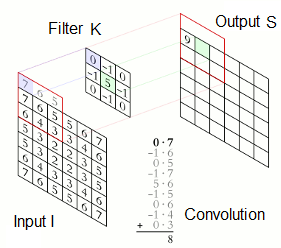
\includegraphics{img/faltung2.png}
			\captionof{figure}{Faltung einer 6x6 Matrix (mit Zero-padding) und einem 3x3 Filter \cite{wikipic}}
			\label{img:faltung}
		\end{minipage}\newline
		\subsubsection*{Convolutional Layer}
		In einem CL findet eine Faltung der Eingangsdaten, in Form einer Matrix und einem oder mehreren Filtern, statt. Ein Filter dient, beispielsweise zur Glättung oder zur Verkleinerung, der Daten. Eine Verkleinerung der Eingangsmatrix findet statt, wenn ein Filter ohne Zero-padding\footnote[11]{Eine Matrix wird, bei einer Faltung, am Rand, um Nullen erweitert. Bsp. aus einer 7x7 Matrix wird eine 9x9 Matrix} verwendet wird. Die Parameter eines Filters werden zufällig initialisiert, können aber, mit Hilfe des Backpropagation Verfahrens, vgl. Kapitel 3.1.2, angepasst werden. Werden mehrere Filter auf die Eingangsdaten angewendet, ändert sich die Tiefe der gesamten Ausgangsmatrix entsprechend der Anzahl der Filter. \cite{karpathy}\newline
		In Abbildung \ref{img:faltung} ist die Eingabematrix \textit{I} eine 6x6 Matrix und \textit{K} ein 3x3 Filter. Die Ausgabematrix \textit{S} wir an den Stellen (i,j), durch die nachfolgende Gleichung, berechnet. Eine genauere Herleitung der Gleichung findet der Leser u. a. bei \cite{goodfellow}(328f).\newline\\	
		\begin{equation*}
		S(i,j) =(I \star K)(i,j)
		\end{equation*}
		\begin{equation*}
		(I \star K)(i,j) =\newline\sum_{m}^{}\sum_{n}^{}I(i+m,j+n)K(m,n)
		\end{equation*}\newline
		\subsubsection*{Pooling Layer}
		Ein PL wird zwischen zwei CL eingefügt. Ihre Funktion besteht darin, die Größe der Daten zu reduzieren und damit die Anzahl der Parameter für das nächste CL. Durch die Reduzierung wird die Berechnung des gesamten Netzwerkes beschleunigt. \cite{karpathy}\newline Ein PL wandelt die Ausgabe eines CL, durch eine statistische Zusammenfassung von nebeneinander liegenden Ausgängen, um. Verschiedene Methoden für ein Pl sind: Max Pooling \cite{zhou}, eine Übergabe der größten Zahl in einem rechteckigen Umfeld; die Durchschnittsberechnung des Umfeldes oder ein gewichteter Durchschnitt, basierend auf der Entfernung eines zentralen Punktes \cite{goodfellow}(355).\newline
		Abbildung \ref{img:pooling} zeigt einen 2x2 Max-Filter, der auf eine 4x4 Datenmatrix angewandt wird. Die Verschiebung oder Stride des Filters ist 2 dh. der Filter wird zunächst auf der y-Achse verschoben. Erreicht er dort das Ende, wird er um eine Stride auf der x-Achse verschoben und beginnt wieder mit der y-Verschiebung.\newline\\
		\begin{minipage}{0.4\textwidth}
			\centering
			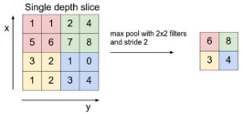
\includegraphics{img/pooling.png}
			\captionof{figure}{Maxpooling mit einem 2x2 Filter\cite{karpathy}}
			\label{img:pooling}
		\end{minipage}\newline
		\subsubsection*{Fully-Connected Layer}
		Ein oder mehrere geschachtelte FCL dienen als Ausgabeschicht. Jeder Knoten in einer FCL, hat eine Verbindung, zu allen Knoten, der vorherigen Schicht. Abhängig von der Problemstellung, Klassifizierung oder Regression, ist die Anzahl der Ausgabeknoten unterschiedlich. Bei einer Klassifizierung entspricht die Anzahl, in der letzten FCL, der der Klassen, die das CNN unterscheiden soll. Die Ausgabe der FCL ist ein Vektor in der jeder Eintrag, die Wahrscheinlichkeit, der jeweiligen Klasse, spiegelt. Bei einer Regression gibt das FCL einen oder mehrere Realwerte aus. \cite{karpathy}
		\subsubsection{Training}
		CNNs werden, durch die Backpropagation Methode, trainiert. Backpropagation basiert auf dem Gradientenverfahren, welches versucht für die Fehlerfunktion \textit{E}, durch sukzessive Iteration der Parameter, ein globales Minimum zu finden, meistens aber nur ein lokales findet. Um das Minimum zu erreichen, werden die Werte der Gewichte \textit{w}\textsubscript{ij}, durch Verwendung der Kettenregel, der partiellen Ableitung, berechnet\footnote[12]{Ausgabeparameter \textit{o}, beliebige Anzahl an Knoten \textit{net} zwischen Ausgabe und \textit{w}}:
		\begin{equation*}
		\centering
		\frac{\partial\textit{E}}{\partial\textit{w}\textsubscript{ij}} = \frac{\partial\textit{E}}{\partial\textit{o}\textsubscript{j}} \frac{\partial\textit{o}\textsubscript{j}}{\partial\textit{net}\textsubscript{j}}  \frac{\partial\textit{net}\textsubscript{j}}{\partial\textit{w}\textsubscript{ij}} 
		\end{equation*}\newline
		Der neue Wert eines Parameters \textit{w}, zum Zeitpunkt \textit{t}, lässt sich durch folgende Formel, berechnen:
		\begin{equation*}
		\centering
		\textit{w}(\textit{t}) = \textit{w}(\textit{t}-1) + \eta * \frac{\partial\textit{E}}{\partial\textit{w}} 
		\end{equation*}
		Die Lernrate $\eta$ ist eine Konstante, die definiert werden muss.\newline
		Anhand der Kostenfunktion, kann die Parameteranpassung und damit der funktionale Wert eines CNN, mit reellen Zahlen, dargestellt und verglichen werden. Diese Funktion \textit{C} lässt sich durch die Summe, über Trainingsbeispiele \textit{m} und einer Fehlerfunktion \textit{E}, hier die negativ conditional Log-Likelihood\footnote[13]{Abgeleitet von Maximum Likelihood, Dichtefunktion für Maximafindung}, darstellen: 
		\begin{equation*}
		\centering
		E(x,y) = -log p(y|x)
		\end{equation*}
		\begin{equation*}
		\centering
		\textit{C} = \frac{1}{m}\sum_{i=1}^{m}E(x\textsuperscript{i},y\textsuperscript{i})
		\end{equation*}
		Das Training eines Netzes ist abgeschlossen, wenn die Kostenfunktion minimal ist bzw. in einem gegebenen Zeitraum, keine bessere gefunden wird. \cite{goodfellow}(80ff,129ff)
		
		\subsection{Anwendung eines CNN zur automatischen Musikempfehlung}
		Dieser Ansatz wird wie folgt umgesetzt: das Netz wird darauf trainiert latente Faktoren, also Eigenschaften, aus einzelnen Musikstücken zu generieren, welche für eine Empfehlung verwendet werden. Dieses Verfahren wird anschließend im Vergleich mit einem konventionellen Ansatz, welcher dem Bag-of-Words Prinzip folgt, betrachtet. Daraus folgend wird beurteilt, inwiefern mittel CNN Eigenschaften zur Spezifizierung des Nutzergeschmacks generiert und ausgewertet werden können.
		
		\subsubsection{Datenbasis}
		Als Datenbasis zur Umsetzung dieses neuen Ansatzes wurden Datensätze des Million Song Dataset (MSD) verwendet, der Echo Nest Taste Profile Subset (ENTPS), sowie der The Last.fm Datensatz. Das MSD verfügt über Metainformationen und bereits analysierter Audio Informationen von Liedern. Ebenso ist dieses öffentlich zugänglich und kann kostenlos heruntergeladen werden. Des weiteren stellt dieses derzeit die größte Forschungsdatenbasis im Gebiet der Musikanalyse dar. Da bei diesen Datensätzen keine Roh-Musikdaten mitgeliefert werden, wurden für die einzelnen Lieder jeweils 29 Sekunden Ausschnitte von der Seite 7digital.com genutzt.\cite{MillionSongDataset} \cite{oord}
		
		\subsubsection{Weighted matrix factorization}
		Der ENTPS Datensatz enthält, die Abspielhäufigkeit eines Songs für jeden Nutzer, also eine implizite Bewertung des Nutzer für diese Lieder. Allerdings kann für ein Musikstück, für einen oder mehrere Nutzer, auch keine Bewertung vorliegen. Dieser Umstand, dass ein Lied keine Wertung erhalten hat, kann mehrere Gründe haben, unter anderem das ein Nutzer dieses Lied schlicht und ergreifen nicht kennt. Der Nutzer könnte allerdings das Lied bereits kennen, aus anderen Quellen, es nicht mögen und deshalb diesen Titel nicht anhören. Dies führt zu zwei unterschiedlichen Szenarien auf Grundlage der gleichen Wertung. Um diesen Umstand richtig bewerten zu können, muss der verwendete Algorithmus flexibel sein. Deshalb kommt ein weighted matrix factorization (WMF) Algorithmus zum Einsatz, um die Informationen aus dem ENTPS trainieren zu können. \cite{oord} Diese Idee ist angelehnt an den Versuch bei der Bewertung von Fernsehshows und deren automatisierter Empfehlung, dem Nutzer gegenüber, möglichst gute Ergebnisse zu erzielen. Es wurde gespeichert wie oft ein Nutzer ein Fernsehformat angesehen hat. Auch hier tritt der Fall auf das für Formate von einzelnen Nutzern keine Bewertungen vorlagen. Dies kann mehrere Gründe haben: der Nutzer kennt das Format nicht, eine Sendung die er noch mehr schätzt kommt zur gleichen Sendezeit oder er mag die Sendung nicht. Folglich gibt es auch hier eine Ausgangswertung und drei Verschiedene Schlussfolgerungen sind möglich. \cite{CollaborativeTVShow}\newline
		Dieser, für implizite Bewertungen optimierte, Algorithmus ist wie folgt aufgebaut:
		
		\begin{equation*}
		\textit{p\textsubscript{ui}} = I(\textit{r\textsubscript{ui}} > 0),
		\end{equation*}
		\begin{equation*}
		\textit{c\textsubscript{ui}} = 1 + \alpha \log (1 + \epsilon\textsuperscript{-1} \textit{r\textsubscript{ui}})
		\end{equation*}\newline\\
		\textit{r\textsubscript{ui}} ist die Anzahl wie häufig ein Lied \textsubscript{i} durch den Nutzer \textsubscript{u} gehört wurde. Für jedes dieser Datenpaare, wird eine Präferenz Variable \textit{p\textsubscript{ui}} definiert. Sie indiziert ob der Nutzer das Lied jemals angehört hat, entspricht der Wert, der Variable, 1 dann wird ausgegangen der Nutzer mag das Lied. Die zweite Variable \textit{c\textsubscript{ui}}, zeigt an wie stark die Bewertung des Liedes in das Empfehlungssystem einfließen soll. Lieder mit höheren Spielraten, werden stärker berücksichtigt, der Wert von \textit{c\textsubscript{ui}} ist hoch, da man sich hier sicherer ist dass, der Nutzer, das Lied mag. Lieder mit geringen Spielraten werden mit einem niedrigen Wert für \textit{c\textsubscript{ui}} bedacht.
		$\alpha$ und $\epsilon$ sind Hyperparameter.
		
		Die Zielfunktion der WMF ist wie folgt gegeben:
		
		\begin{minipage}{0.2\textwidth}
			\centering
			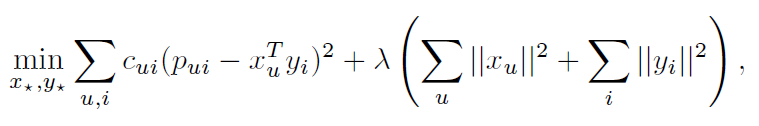
\includegraphics[width=6.5cm]{img/Zielfunktion.png}
		\end{minipage}\newline
		$\lambda$ ist der Regularations-Parameter. \textit{X\textsubscript{u}} stellt den Eigenschafts Vektor des Nutzers \textsubscript{u} dar. \textit{y\textsubscript{i}} den Vektor für das Musikstück \textsubscript{i} dar. Die Zielfunktion besteht aus einem L2 Regularisationsterm und einem Term über die Mittlere Quadratische Abweichung für die bereits erläuterten Variablen. Die Summe im ersten Teil der Funktion beinhaltet jede mögliche Kombination von Nutzern und Liedern, deshalb kommt eine Methode zur Näherung der alternierenden kleinsten Quadrate zum Einsatz. Dieser Ansatz ist ebenfalls an das bereits genannte Verfahren, zur Empfehlung von Fernsehsendungen.\cite{oord} 
		
		\subsubsection{Extraktion und Analyse möglicher Faktoren aus dem Audiosignal}
		Der Akt der Extraktion von Eigenschaften auf Basis von Audiosignalen eines gegeben Liedes, ist ein Regressionsproblem. Dies benötigt das Lernen einer Funktion welche Zeitintervalle auf einen Vektor reeller Zahlen abbilden kann. Um dies zu Lösen, wird ein neuer Ansatz verfolgt: die Nutzung eines CNNs. Die mittels des, berteis erläuterten, WMF Algorithmus gefunden Vektoren auf Basis der vorhanden Daten, werden eingesetzt um das Empfehlungssystem zu trainieren.
		Um das Netz gut trainieren zu können, ist es nötig auf eine große Menge an Trainingsdaten zurückgreifen zu können. Dies wird mittels der MSD, welche bereits vorgestellt wurde, abgesichert. 
		Die Geschwindigkeit des Trainings an sich wird als kritisch betrachtet. Um ein schnelles Lernen zur ermöglichen, wurde der Lernvorgang parallelisiert und mittels GPU Unterstützung zur Berechnung optimiert. Eine GPU ist im Vergleich zu einer CPU in der Lage, in der gleichen Zeit, deutlich mehr Operationen durchzuführen, welche zum trainieren eines Neuronalen Netzes nötig sind.\newline\\		
		Das Trainining des CNN erfolgte in folgenden Schritten: Als erstes wurden aus den Audiosignalen Zeit-Freuqzenz-Details extrahiert, um diese als Input für das Netz zu verwenden Dies erfolgte durch logarithmisch komprimierten Mel-Spektogramme welche aus 128 Komponenten bestehen. Das Netz wurde mit 3 Sekundenlangen Audioschnipseln trainiert, welche zufällig aus den Songs entnommen wurden, dies sorgte für eine zusätzliche Beschleunigung der Trainingsgeschwindigkeit. Um die Features für den gesamten Song zu ermitteln wurden die Faktoren von aufeinanderfolgenden 3-Sekunden-Musikschnipseln gemittelt. Da als Ergebnis der Zielfunktion die Faktoren als reelle Werte benötigt werden, muss der Quadratische Mittlere Fehler der vorhersagen reduziert werden. Alternativ wurde auch eine Verbesserung der Genauigkeit der WMF Zielfunktion betrachtet. \cite{oord}
		
		\subsubsection{Versuch und Durchführung vergleichender Tests}
		Um die Leistungsfähigkeit des neuen Ansatzes auf Basis eines neuronalen Netzes darlegen zu können, wurde ein Experiment mit diesem durchgeführt. Auch wurde ein klassisches Modell, basierend auf dem bereits erläuterten BoW Ansatz umgesetzt, um die Ergebnisse vergleichen zu können. Um die Qualität der Empfehlungen aber auch die extrahierten Faktoren an sich untersuchen zu können, wurden folgende Schritte unternommen.\newline\\
		Um die Vielseitigkeit der extrahierten Audio-Features zu untersuchen, wurden diese, mit Tags für Lieder aus einem Tag-Prediktion-Verfahren verglichen. Tags können Songs beschreiben, unter anderem Genre, Instrumentierung, Tempo, Stimmung und Erscheinungsjahr. Dieser Vergleich wurde auf Basis aller 9,330 Lieder des Last.fm Datensatzes erstellt und die 50 Beliebtesten Tags für jedes Lied extrahiert. Der Vergleich ergab das die Vektoren einen erhöhte Empfehlungsgenauigkeit erbringen.\newline
		Um quantitativ zu beurteilen, wie gut die aus den Audioquellen der Lieder den Liedern extrahiert Faktoren  werden können wurden die Vorhersagen verwendet um damit diesem für ein Empfehlungssystem umzusetzen. Für jeden Nutzer \textsubscript{u} und jeden Song textsubscript{i} der Datenbasis wurde eine Wertung \textit{x\textsuperscript{T}\textsubscript{u}}\textit{y\textsubscript{i}} errechnet und das Lied mit dem höchten Wert als erstes vorgeschlagen. Zum Vergleich wurde ebenfalls eine Metrik auf Basis von Liederähnlichkeiten mittels Bag-of-Words System gelernt um Vorschlagsbewertunge zu erhalten. In diesem Modell wurden alle Wertungen für einen gegebenen Nutzer in eine Durchnschnitts-Ähnlichkeits-Wertung umgerechnet basierend auf alle Lieder welche dieser Nutzer bereits hörte.\newline\\
		Um die Vektoren zur Empfehlung generieren zu können, wurde jeweils Folgende Ansätze verfolgt:
		Eine Lineare Regression welche auf den Bag-Of-Words Ansatz trainiert wurde.
		Ein mehrlagigen Perzeptron, ein vereinfachtes künstliches Netz,  trainiert auf ebenfalls das gleiche BoW-Modell. \cite{perceptron}
		Ein CNN, welches auf log-skalierten Mel-Spektogrammen trainiert wurde, um den den Mittleren quadratischen Fehler der Vorhersagen zu reduzieren. 
		Sowie das gleiche CNN trainiert um den Empfehlungen aus dem WMF zu verbessern. \cite{oord}\newline\\
		In ersten Experimenten wurden nur Teilmengen der vorhanden Datensätze genutzt. Betrachtet man die Durchschnittsgenauigkeit der Empfehlungssystem ergibt sich folgendes Bild:  Die lernenden Ansätze sind Leistungsfähiger als die Lineare Regression. Selbst der Ansatz basieren auf dem Perzeptron erweist sich als besser, als das Regressionsmodell. Die beiden auf CNN basierenden Modelle sind deutlich besser im Vergleich zu den beiden erstgenannten Modellen. Die vergrößerung der Datenbasis für weitere Experimente lässt die Leistungsfähigkeit und den Leistungsvorsprung der beiden auf CNN basierenden Ansätze noch größer werden. \cite{oord}\newline\\
		Eine Bewertung der Qualität der gefundenen Vektoren, kann nicht nur durch Metriken bestimmt werden. Ein Vergleich der mittels CNN vorhergesagten Vektoren empfohlenen Liedern einerseits und empfehlungen eines 50-dimesionalen WMFs anderseits ergaben folgendes: die empfohlenen Lieder sind zumeist unterschiedlich, nur wenige Teilmengen vorhanden. Allerdings erbringen beide Modelle ein gutes Ergebnis und die mittel CNN-Modell vorgeschlagenen Auswahl an Liedern ist etwas abwechslungsreicher was für ein Empfehlungssystem als Vorteil zu sehen ist. \cite{oord}
		
		\subsection{Hybride Musikempfehlung mit einem Neuronalen Netzwerk}
		Im Unterschied, zu der davor dargestellten Forschung in Kapitel 3.2, wird nun ein Deep Belief Netzwerk (DBN) verwendet, um ein hybrides inhaltsbasiertes Musikempfehlungssystem zu entwickeln. Im Gegensatz zu einem CNN, nutzt ein DBN ein so genanntes Pretraining\footnote[14]{Parameter von Model A wird für das neue Model B verwendet} als Parameterinitialisierung. Bisherige inhaltsbasiertes Systeme verfolgen typischerweise einem zweistufigen Ansatz: Zunächst extrahieren sie aus Audioinhalte den MFCC Koeffizienten; anschließend prognostizieren sie Musikpräferenzen, eines Nutzers. Das nachfolgende Modell führt diese beiden Schritte simultan und automatisch aus. \cite{wang}\newline
		Das hybride Modell basiert auf einem hierarchisch linearen Modell mit einem Deep Belief Netzwerk (HLDBN), das zunächst erläutert wird, um anschließend die Funktionsweise, des hybriden Systems, darzustellen.
		\begin{minipage}{0.45\textwidth}
			\centering
			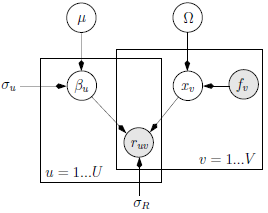
\includegraphics{img/hlmdbn.png}
			\captionof{figure}{Hierarchisches lineares Modell eins Deep Belief Netzwerks \cite{wang}}
			\label{img:hlmdbn}
		\end{minipage}
		\subsubsection{Hierarchisch lineares Modell mit einem Deep Belief Netzwerk}
		Das in Abbildung \ref{img:hlmdbn} gezeigte Modell ist wie folgt definiert: \textit{f\textsubscript{v}} sind Musikmerkmale eines Liedes \textit{v}, die durch den Merkmalsvektor x\textsubscript{v} automatisch errechnet werden. Die bevorzugte Musik eines Benutzers \textit{u}, wird als Vektor $\beta$\textsubscript{u} bezeichnet. $\Omega$ bezeichnet die Parameter, die das DBN lernt. Die Bewertung \textit{r\textsubscript{xv}}, die ein Nutzer einem Lied \textit{v} gibt, ist ein Skalarprodukt von \textit{x\textsubscript{v}} und $\beta$\textsubscript{u}. Durch $\sigma$\textsubscript{R} wird die Varianz aller Bewertungen des Nutzers betrachtet. $\mu$ repräsentiert den allgemeinen Musikgeschmack aller Benutzer, wobei $\sigma$\textsubscript{u} die Varianz des einzelnen Nutzers definiert. Alle Benutzer und Lieder Paare werden als \textit{I} bezeichnet. Für eine Regularisierung der Werte wird die Gaußsche Normalverteilung $\mathcal{N}$ verwenden.\footnote[15]{$\mathcal{N}$(a,b) ist die Normalverteilung mit Mittelwert a und Varianz b. x $\sim$ p zeigt, dass x die Verteilung p erfüllt}\newline
		Das Modell ist wie folgt formuliert:\newline
		\begin{equation*}
		\centering
		\textit{r\textsubscript{xv}}\sim\mathcal{N}(\beta'\textit{x\textsubscript{v}},\sigma\textsuperscript{2}\textsubscript{R})
		\end{equation*}
		\begin{equation*}
		\centering
		\beta\sim\mathcal{N}(\mu,\sigma\textsuperscript{2}\textsubscript{u}\textit{I})
		\end{equation*}
		\begin{equation*}
		\textit{x\textsubscript{v}} = DBN(\textit{f\textsubscript{v}};\Omega)
		\end{equation*}\newline\\
		Für das Training des Systems wird im Unterschied zu einem CNN zunächst ein unsupervised\footnote[16]{Ausgabeergebnisse der Testdaten sind nicht vorhanden} Training durchgeführt um die Knoten zu initialisieren. Anschließend findet ein supervised Training zur Optimierung der Parameter statt. Als Optimierungsmethode wird das stochastische Mini-Batch\footnote[17]{nur ein kleiner Teil der vorhandenen Daten wird trainiert} Verfahren mit Backpropagation genutzt, um ein Overfitting\footnote[18]{Spezialisierung} des Modells zu vermeiden. Nach der Lernphase kann die Bewertung \textit{r\textsubscript{xv}} eines Benutzers \textit{u} über ein Lied \textit{v} geschätzt werden, wodurch diesem neue Lieder empfohlen werden können. \cite{wang}
		\subsubsection{Hybrides Modell mit einem Deep Belief Netzwerk}
		Basierend auf dem HLDBM, wird das in Abbildung \ref{img:hybrid} gezeigte Modell, um einen kollaborative Filter erweitert, wodurch eine noch bessere Empfehlungsrate erreicht wird.
		\begin{minipage}{0.45\textwidth}
			\centering
			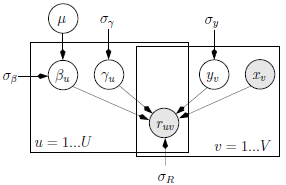
\includegraphics{img/hybrid.png}
			\captionof{figure}{Hybrides Empfehlungs Modell \cite{wang}}
			\label{img:hybrid}
		\end{minipage}\newline\\
		Die Musikmerkmale eines Liedes \textit{x}\textsubscript{v} wird wie in Kapitel 3.4.1 berechnet. Die bevorzugte Musik eines Nutzers, wird als $\beta$\textsubscript{u} bezeichnet. Der kollaborative Teil: $\gamma$\textsubscript{u} stellt einen Vektor über alle Benutzer \textit{u} dar; \textit{y}\textsubscript{v} den Vektor über alle Lieder \textit{v}. $\beta$\textsubscript{u}, $\gamma$\textsubscript{u} und \textit{y}\textsubscript{v} werden gemeinsam, durch das Neuronale Netzwerk, anhand der Trainingsdaten gelernt. Die dazu verwendeten Fehlerfunktionen sind in \cite{wang} beschrieben. Die Empfehlungsrate \textit{r}\textsubscript{uv} ergibt sich aus der Summe der Skalarmultiplikationen  $\gamma$'\textsubscript{u}\textit{y}\textsubscript{v} und  $\beta$'\textsubscript{u}\textit{x}\textsubscript{v}. Die A-priori-Wahrscheinlichkeiten\footnote[19]{Anfangswahrscheinlichkeiten} werden durch, die folgenden Formeln definiert:\newline
		\begin{equation*}
		\centering
		\textit{r\textsubscript{xv}}|\beta\textsubscript{u},\textit{x}\textsubscript{v},\gamma\textsubscript{u},\textit{y}\textsubscript{v},\sigma\textsubscript{R}\sim\mathcal{N}(\beta'\textsubscript{u}\textit{x}\textsubscript{v} + \gamma'\textsubscript{u}\textit{y}\textsubscript{v},\sigma\textsubscript{R}\textsuperscript{2})
		\end{equation*}
		\begin{equation*}
		\centering
		\beta\textsubscript{u}|\sigma\textsubscript{$\beta$}\sim\mathcal{N}(\mu,|\sigma\textsubscript{$\beta$}\textsuperscript{2}I)
		\end{equation*}
		\begin{equation*}
		\centering
		\gamma\textsubscript{u}|\sigma\textsubscript{u}\sim\mathcal{N}(0,|\sigma\textsubscript{$\gamma$}\textsuperscript{2})
		\end{equation*}
		\begin{equation*}
		\centering
		\textit{y}\textsubscript{v}|\sigma\textsubscript{v}\sim\mathcal{N}(0,|\sigma\textsubscript{y}\textsuperscript{2})
		\end{equation*}\newline
		Die Fehler Funktion des Modells wird auch mit Hilfe der Backpropagation minimiert. Um Zeit zu sparen, können die Werte für $\gamma$\textsubscript{u} und \textit{y}\textsubscript{v} durch eine PMF berechnet und als Initialwerte verwendet werden. \cite{wang}\newline
		Um Informationen aus einem Lied, als Eingabeparameter für das DBN, nutzen zu können, müssen diese in einen Vektor umgewandelt werden. Dies geschieht in verschiedenen Schritten. In \cite{wang} werden alle Lieder in ein .wav Dateiformat, mit einer 8 kHz Abtastrate und 16 Bit Tiefe, umgewandelt. Aus den einzelnen Liedern wird ein 5 Sekunden Abschnitt genutzt, der in ein 166x120 Spektrogramm umgewandelt wird. Anschließend wird eine Hauptkomponentenanalyse\footnote[20]{Zusammenhang der Darstellung einer Menge an Variablen durch wenige Faktoren} durchgeführt, wodurch sich ein Vektor für den Liedabschnitt ergibt.
		\section{Vergleich der vorgestellten Modelle}
		Abschließend wird nun ein Vergleich zwischen dem vorgestellten CNN Ansatz einerseits und dem danach folgendem DBN gezogen. In Versuchen \cite{oord} wurde festgestellt das dass CNN Model einem BOW System überlegen ist und eine bessere Empfehlungsrate erreicht. Das anschließend erläuterte  Versuchsmodel, welches mittels DBN einen hybriden Methode verfolgt, konnte im direkten Vergleich zu CNN eine nochmals verbesserte Empfehlungsgenauigkeit erreichen. Vergleichende Versuchsreihen \cite{wang} haben folgendes festgestellt: ein nicht hybrider Ansatz, welcher allein auf Training der beiden Netze basiert, ergab, dass das vorgestellte HLDBN Modell genauere Ergebnisse lieferte als das vorgestellte CNN. Die Integration der beiden Modelle in einen hybriden Aufbau ergab wiederum ebenso dass der Einsatz des HLDBN Netzes zu genaueren Empfehlungsraten führt, als die Verknüpfung von CNN und CF. Die Empfehlungsraten für bereits bekannte Lieder, konnten somit im Vergleich zu klassischen Ansätzen verbessert werden. Auch das bereits eingeführte Problem des NSP konnte durch den Einsatz Neuronaler Netze gelöst werden. Sowohl der Einsatz des CNN als auch der des HLDBN Netzes führen hierbei zum Erfolg. Das ebenfalls bereits vorgestellte NUP konnte dagegen nicht gelöst werden, da in desem Modellen derzeit keine Möglichkeit besteht aus einem, dem System unbekannten, Nutzer Merkmale für eine Vektordarstellung zu generieren. Während aus einem Lied, durch die vorgestellten Modelle Audiofeatures extrahiert und dem System zugeführt werden können.
		Sowohl der in Kapitel 3.2 vorgestellte Ansatz mittels eines CNNs, sowie der in Kapitel 3.3 erläuterte Ansatz mit Einsatz eines hybriden DBN Netzwerkes eine gute Möglichkeit zur automatisierten Musikempfehlung. Beide Verfahren haben in Rahmen von Versuchen bewiesen, dass sie sowohl zuverlässig sind und durch bessere Empfehlungsraten einem klassischen Ansatz überlegen sind.
		%\bibliographystyle{abbrvdin}
		\bibliographystyle{unsrt}
		\bibliography{lit}
	\end{multicols}
\end{document}
